%% IMPORTANT: Once working, run latex 3 times to get listoffigures to work

%% Be sure to check spelling!

%% Put your name and the proper due date in place

%% Copy the lstinputlisting and figure code as many times as you need
%% Be sure to put in your own file names if appropriate

%% Note that the \epsfig and \lstinputlisting commands 
%% are currently commented out with %%% - until the
%% files exist, processing this code without them will result in an error
%% so leave the comments until you have created the files!

\documentclass{article}
\usepackage{amsmath}    % loads AMS-Math package
\usepackage{epsfig}     % allows PostScript files
\usepackage{listings}   % allows lstlisting environment
\usepackage{moreverb}   % allows listinginput environment
\usepackage[letterpaper, margin=0.75in]{geometry}  % set paper size/margins
\usepackage{EGR103F19}  % colorful file imports

\begin{document}
\begin{center}
\rule{6.5in}{0.5mm}\\~\\
\textbf{\large EGR 103L -- Fall 2019}\\~\\
\textbf{\huge Functions and Random Numbers}\\~\\
***NAME (NetID)***\\
***Lab Section N, DAY TIMES***\\
***DATE DUE***\\~\\
{\small I understand and have adhered to all the tenets of the Duke
  Community Standard in completing every part of this assignment.  I
  understand that a violation of any part of the Standard on any part
  of this assignment can result in failure of this assignment, failure
  of this course, and/or suspension from Duke University.} 
\rule{6.5in}{0.5mm}\\
\end{center}
\tableofcontents
\listoffigures
\pagebreak

\section{P\&E 1.31 - Time}
%%% \lstinputlisting{time_diary.txt}

\section{Reworked P\&E 1.31 - More Time}
%%% \lstinputlisting{seconds_diary.txt}

\section{P\&E 1.35 - Triangles}
%%% \lstinputlisting{tri_diary.txt}

\section{P\&E 1.39 - Football}
%%% \lstinputlisting{passer_diary.txt}

\clearpage

\section{Random Integers}
%%% \lstinputlisting{dice_diary.txt}

\section{Random Numbers}
\begin{lstlisting}
%%% Paste from screen here
\end{lstlisting}

\pagebreak
\appendix
\section{Codes}
% change all listings to python style 
\lstset{style=python103, language=python} 

% Put the name of your file in the subsection name 
% and the listinginput input
% Be sure to include the community standard in codes!

% Add \clearpage if it makes sense

% Put the files in the same order as the problems

% Be sure to remove %%% from lstinputlisting lines!

\subsection{keep\_time.py}
\lstinputlisting{keep_time.py}

\subsection{get\_time.py}
\lstinputlisting{get_time.py}

\subsection{tri\_cal.py}
\lstinputlisting{tri_calc.py}

\subsection{football.py}
\lstinputlisting{football.py}

\subsection{play\_game.py}
\lstinputlisting{play_game.py}

\subsection{gen\_rand.py}
\lstinputlisting{gen_rand.py}

\clearpage % start Figures on new page

\section{Figures}
% Don't forget to take out %%% on epsfig lines!

\begin{figure}[ht!]
\begin{center}
\begin{tabular}{cc}
%%% \epsfig{file=TriPlotTest1.eps, width=3in} & 
%%% \epsfig{file=TriPlotTest2.eps, width=3in} \\ 
%%% \epsfig{file=TriPlotTest3.eps, width=3in} & 
%%% \epsfig{file=TriPlotTest4.eps, width=3in} \\ 
\end{tabular}
\end{center}
\caption{Test Triangles.}
\end{figure}
\pagebreak

\begin{figure}[ht!]
\begin{center}
%%% 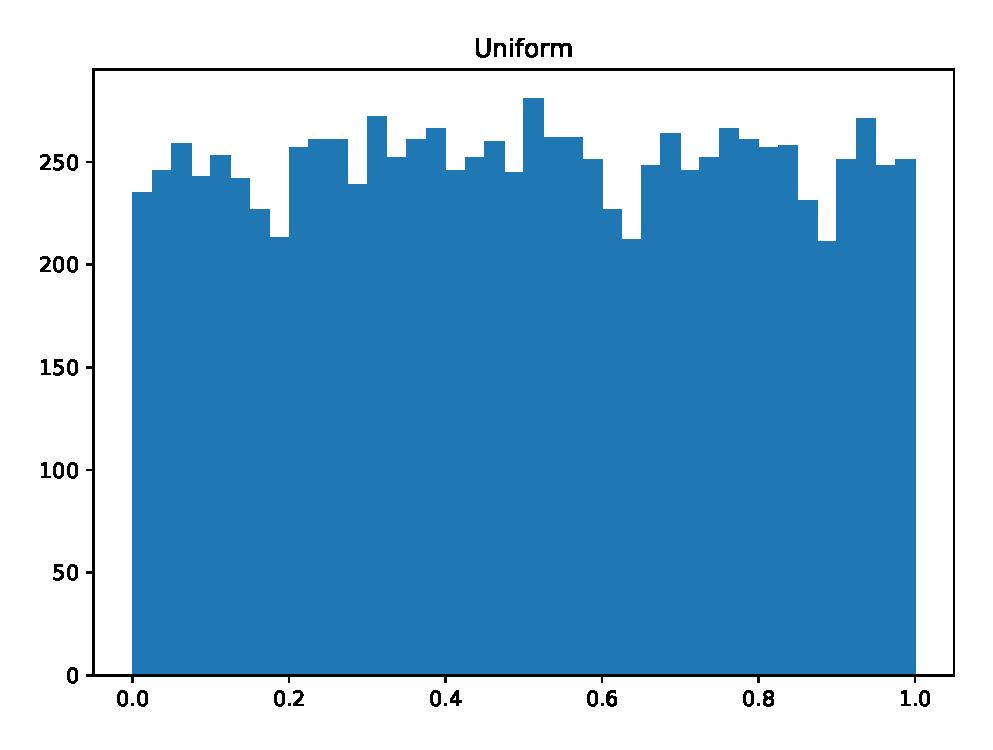
\epsfig{file=UniformPlot.eps, width=4.5in}
\caption{Histogram of Uniformly Distributed Random Numbers.}
\end{center}
\end{figure}

\begin{figure}[ht!]
\begin{center}
%%% 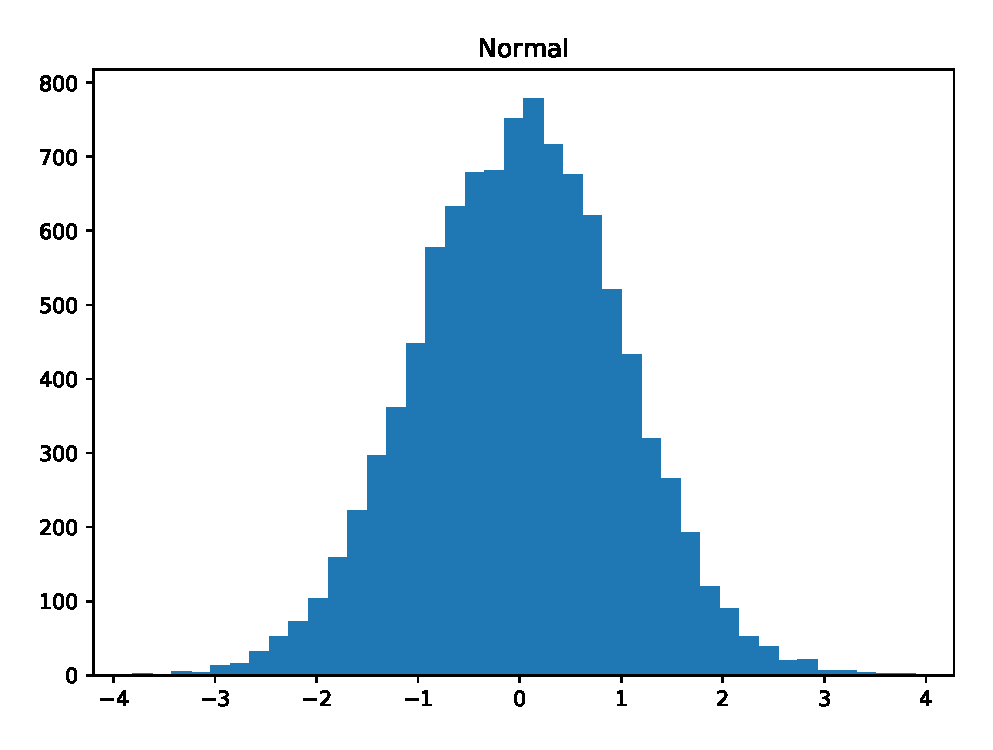
\epsfig{file=NormalPlot.eps, width=4.5in}
\caption{Histogram of Normally Distributed Random Numbers.}
\end{center}
\end{figure}
\end{document}
